

\begin{figure}[h!]
    \centering
    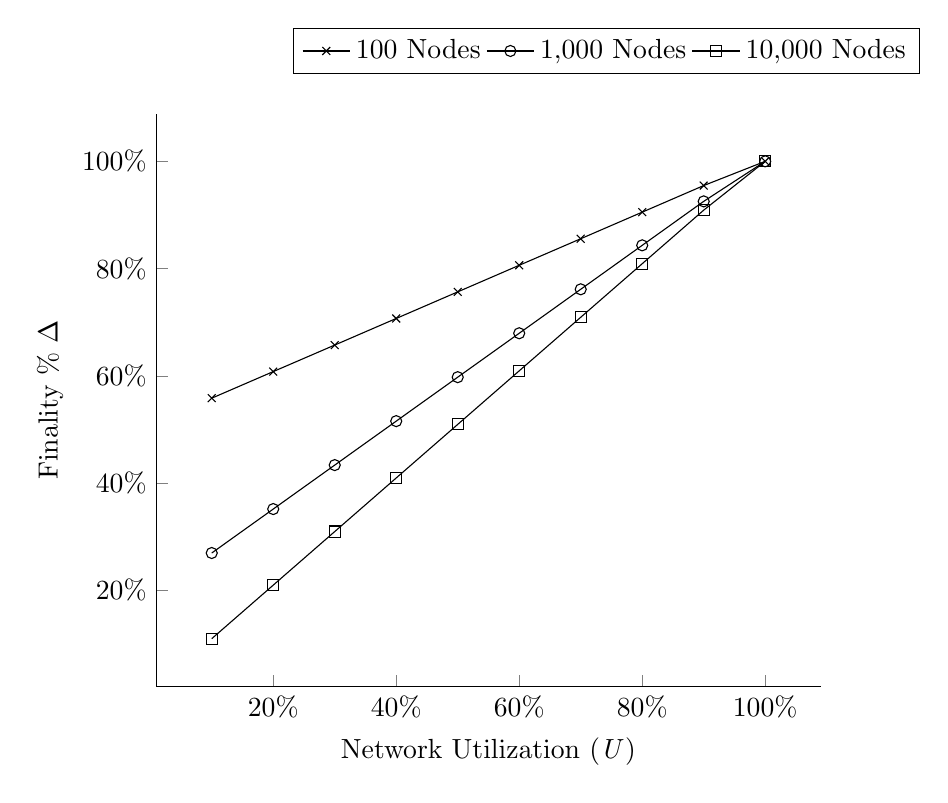
\begin{tikzpicture}
      \pgfplotsset{
          scale only axis,
          xticklabel={\pgfmathparse{\tick*100}\pgfmathprintnumber{\pgfmathresult}\%},
          yticklabel={\pgfmathparse{\tick*100}\pgfmathprintnumber{\pgfmathresult}\%},
          every axis legend/.append style={ at={(1.15,1.15)}, 
          legend columns = 0}
          % legend style={at={(0.5,0.5)},
      }
    
      \begin{axis}[
        % xmode=log,
        % ymode=log,
        axis y line*=left,
        axis x line*=bottom,
        xlabel = Network Utilization (\textit{U}),
        ylabel= Finality \(\%\) \(\Delta\),   
        scaled y ticks=true
      ]

        \addplot[mark=x,color=black] coordinates{
            (1, 1)
            (.9,.9548)
            (.8,.9052)
            (.7,.8556)
            (.6,.8061)
            (.5,.7565)
            (.4,.7069)
            (.3,.6573)
            (.2,.6078)
            (.1,.5582)
            % more points
          }; \label{plot_1_y1}
    
        \addplot[mark=o,color=black] coordinates{
            (1, 1)
            (.9,.9253)
            (.8,.8433)
            (.7,.7613)
            (.6,.6793)
            (.5,.5974)
            (.4,.5154)
            (.3,.4334)
            (.2,.3514)
            (.1,.2694)
            % more points
          }; \label{plot_1_y2}
          
        \addplot[mark=square,color=black] coordinates{
            (1, 1)
            (.9,.9089)
            (.8,.809)
            (.7,.7091)
            (.6,.6092)
            (.5,.5093)
            (.4,.4094)
            (.3,.3094)
            (.2,.2095)
            (.1,.1096)
            % more points
          }; \label{plot_1_y3}

%           100 %	1	1	1
% 90 %	0.9548	0.9253	0.9089
% 80 %	0.9052	0.8433	0.809
% 70 %	0.8556	0.7613	0.7091
% 60 %	0.8061	0.6793	0.6092
% 50%	0.7565	0.5974	0.5093
% 40 %	0.7069	0.5154	0.4094
% 30 %	0.6573	0.4334	0.3094
% 20 %	0.6078	0.3514	0.2095
% 10 %	0.5582	0.2694	0.1096
        
        \addlegendimage{/pgfplots/refstyle=plot_1_y1}\addlegendentry{100 Nodes}
        \addlegendimage{/pgfplots/refstyle=plot_1_y2}\addlegendentry{1,000 Nodes}
        \addlegendimage{/pgfplots/refstyle=plot_1_y3}\addlegendentry{10,000 Nodes}

        \end{axis}
    \end{tikzpicture}
    \caption{The percentage decrease in finality time as \textit{network utilization} decreases.}
    \label{fig:fin_change}
\end{figure}